% =============================================================================
%  Rapport — « Combien vaut une voiture d'occasion ? »
%  Introduction to Data Processing — MAM3, Université Côte d'Azur, 2025-2026
%  Équipe : Hafssa, Thibaud, Nathan
%
%  Compilation : pdflatex (Overleaf par défaut) ; XeLaTeX/LuaLaTeX aussi (garde iftex).
%      pdflatex report.tex   (×2 pour le sommaire/les références)
% =============================================================================
\documentclass[11pt,a4paper]{article}

\usepackage{iftex}
\ifpdftex
  \usepackage[utf8]{inputenc}
  \usepackage[T1]{fontenc}
\fi
\usepackage[french]{babel}
\usepackage[a4paper,margin=2.5cm]{geometry}
\usepackage{graphicx}
\usepackage{booktabs}
\usepackage{amsmath,amssymb}
\usepackage{xcolor}
\usepackage{caption}
\usepackage{enumitem}
\usepackage[hidelinks]{hyperref}

\graphicspath{{figures/}}

% Couleurs : rouge = fait MONTER le prix, bleu = fait BAISSER le prix.
\definecolor{priceup}{HTML}{2E7D32}
\definecolor{pricedown}{HTML}{C62828}
\newcommand{\priceUp}[1]{\textcolor{priceup}{#1}}    % vert = +cher
\newcommand{\priceDn}[1]{\textcolor{pricedown}{#1}}  % rouge = -cher

\title{\textbf{Combien vaut une voiture d'occasion ?}\\[2pt]
  \large Rapport --- \textit{Introduction to Data Processing} (MAM3, 2025-2026)}
\author{Hafssa \quad\textbullet\quad Thibaud \quad\textbullet\quad Nathan}
\date{Université Côte d'Azur --- Polytech Nice Sophia}

\begin{document}
\maketitle

\noindent\textbf{Dépôt Git :} \url{https://github.com/barbiernathan2005/PROJET-DATA-SCIENCE}\\
\textbf{Dataset :} \textit{100,000 UK Used Car Data} (Kaggle) --- 7 marques fusionnées.

\medskip\hrule\medskip

% =============================================================================
\section{Business goal}
% =============================================================================

\noindent\textbf{Quel est notre dataset ? Pourquoi est-il utile ?}

\medskip
Notre projet répond à une question concrète et universelle : \textbf{peut-on prédire le
prix d'une voiture d'occasion à partir de ses caractéristiques ?} L'enjeu est réel : un
bon modèle aide acheteurs et vendeurs à estimer un prix juste, alimente les plateformes
de petites annonces et permet de \textbf{repérer les bonnes (et les mauvaises) affaires}.

Notre parcours a commencé par un \textbf{échec instructif}. Notre premier dataset
(\texttt{Global\_Mental\_Health\_Dataset\_2025.csv}, \textbf{2\,500 lignes}), sur la
« santé mentale », semblait idéal pour notre première problématique --- \textit{peut-on
prédire le stress à partir du sommeil ?} Mais à l'analyse, \textbf{aucune variable
n'était corrélée à une autre} : la corrélation maximale (hors diagonale) ne valait que
$|r| \approx 0{,}04$, et le couple sommeil\,$\leftrightarrow$\,stress tombait à
$-0{,}01$ (Figure~\ref{fig:synth}). Ces données étaient \textbf{générées
artificiellement}, pas mesurées. Première leçon, devenue notre fil rouge :
\textit{vérifier la provenance et la réalité des données avant toute analyse.}

\begin{figure}[h]
  \centering
  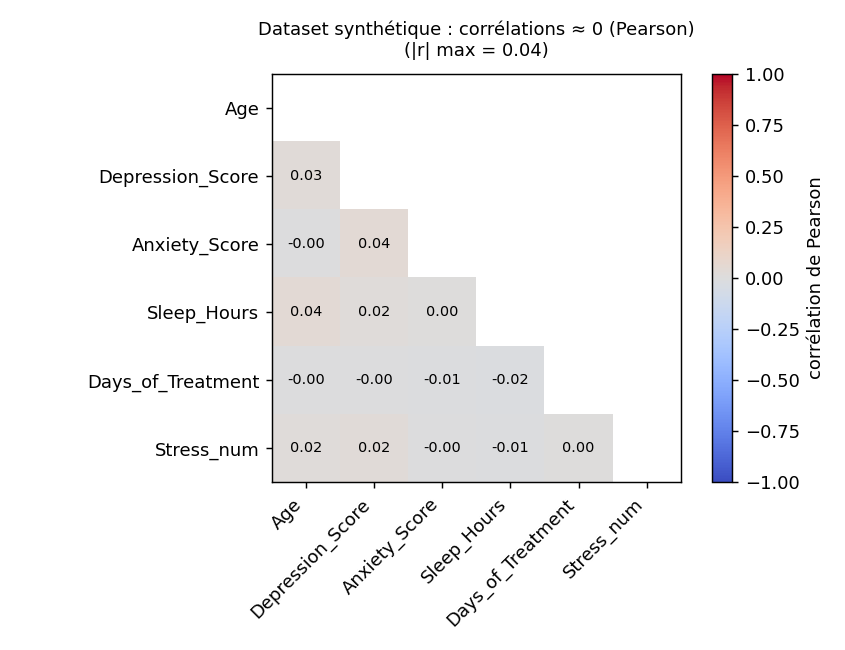
\includegraphics[width=0.6\linewidth]{00_probleme1_synthetique.png}
  \caption{Le dataset abandonné (synthétique). La matrice de corrélation est entièrement
    « éteinte » (toutes les cases $\approx 0$) : c'est la \textbf{signature de données
    fabriquées} --- aucune relation exploitable.}
  \label{fig:synth}
\end{figure}

Nous avons alors choisi un jeu de données \textbf{réel} : le dataset \textit{UK Used
Cars} (annonces réelles de voitures d'occasion au Royaume-Uni, 7 marques : Audi, BMW,
Ford, Hyundai, Skoda, Toyota, Volkswagen). Contrairement au premier, ces données
présentent de \textbf{vraies relations exploitables} --- et les imperfections typiques du
réel (années aberrantes, doublons), gage d'authenticité.

% =============================================================================
\section{Team management}
% =============================================================================

\noindent\textbf{Comment travaillons-nous ? Quel est notre planning ?}

\medskip
Nous sommes une équipe de \textbf{3 personnes}, coordonnée via un \textbf{dépôt Git}
partagé.

\medskip
\noindent\textbf{Répartition des rôles :}
\begin{itemize}[nosep,leftmargin=1.4em]
  \item \textbf{Hafssa --- Données \& nettoyage :} chargement, sanity checks, années
    aberrantes et doublons, encodage des catégories.
  \item \textbf{Nathan --- Visualisation \& features maison :} heatmap, boxplots,
    conception des indices (\texttt{car\_age}, \texttt{mileage\_per\_year}).
  \item \textbf{Thibaud --- Modélisation \& storytelling :} régression linéaire,
    évaluation (R²/RMSE), interprétation, rédaction du récit et des slides.
\end{itemize}

\medskip
\noindent\textbf{Planning (calendrier du cours) :}
\begin{center}
\begin{tabular}{@{}ll@{}}
  \toprule
  \textbf{Jour} & \textbf{Tâche} \\
  \midrule
  Lun.\ 01/06 & Définition du problème, 1\textsuperscript{er} dataset (santé mentale) $\to$ abandon \\
  Mar.\ 02/06 & Choix du dataset réel (voitures), chargement, nettoyage \\
  Mer.\ 03/06 & Features maison, visualisation, régression linéaire \\
  Jeu.\ 04/06 & Évaluation, pipeline final, préparation de l'oral \\
  Ven.\ 05/06 & Soutenance orale + finalisation du rapport \\
  \bottomrule
\end{tabular}
\end{center}

% =============================================================================
\section{Data visualisation}
% =============================================================================

\noindent\textbf{Description.} Le dataset contient \textbf{72\,435 lignes} et
\textbf{10 variables}. La cible est \texttt{price}, le prix de vente en \textbf{livres
sterling (£)}. Les explicatives sont de deux types :
\begin{itemize}[nosep,leftmargin=1.4em]
  \item \textbf{numériques} : \texttt{year}, \texttt{mileage}, \texttt{tax},
    \texttt{mpg} (consommation), \texttt{engineSize} (cylindrée) ;
  \item \textbf{catégorielles} : \texttt{model}, \texttt{transmission},
    \texttt{fuelType} et \texttt{Make} (marque).
\end{itemize}

\noindent\textbf{Nettoyage (data wrangling).} Deux années manifestement erronées
(\texttt{2060} et \texttt{1970}) ont été retirées, ainsi que les \textbf{doublons} : le
dataset passe de \textbf{72\,435 à 71\,593 lignes}. Le carburant \texttt{Electric}, très
rare, a été regroupé dans \texttt{Other}.

\begin{figure}[h]
  \centering
  
\includegraphics[width=0.62\linewidth]{01_heatmap_correlations.png}
  \caption{Heatmap des corrélations (variables numériques). La cylindrée
    \texttt{engineSize} (\priceUp{$+0{,}63$}) et l'année \texttt{year} (\priceUp{$+0{,}52$}) sont
    les plus liées au prix ; le kilométrage (\priceDn{$-0{,}43$}) et l'âge (\priceDn{$-0{,}52$}) le
    tirent vers le bas.}
  \label{fig:heat}
\end{figure}

\begin{figure}[h]
  \centering
  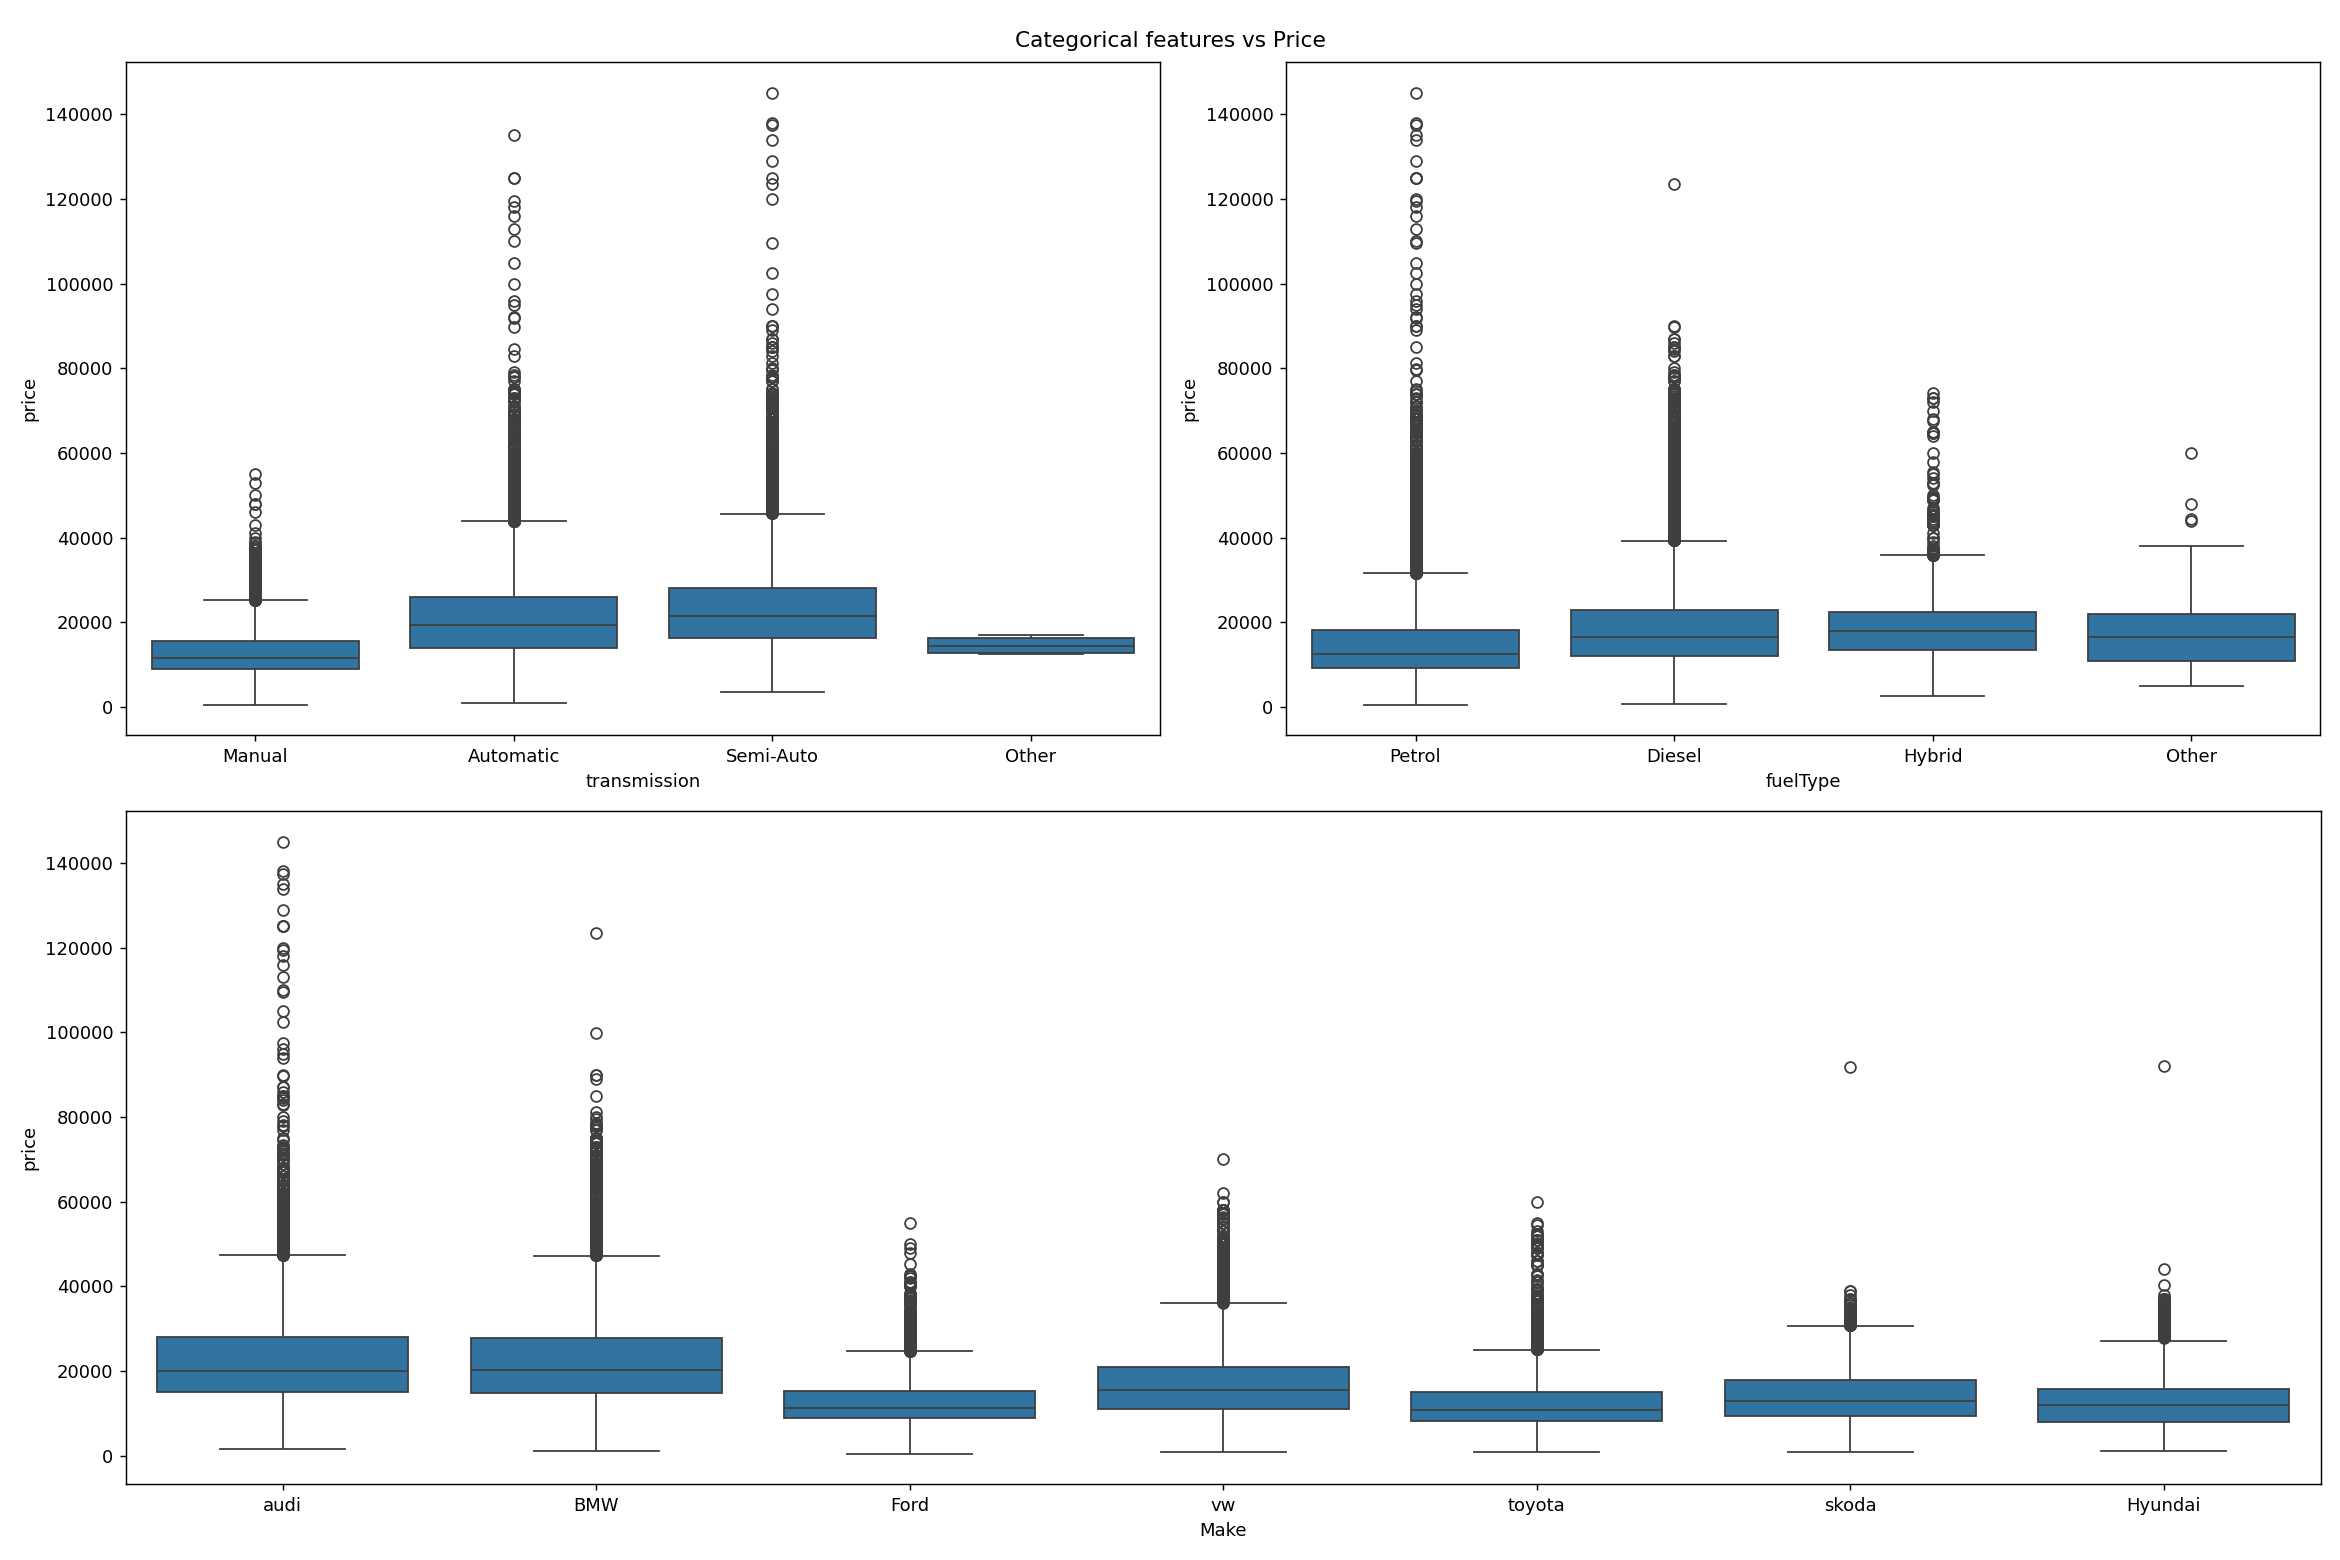
\includegraphics[width=0.78\linewidth]{02_prix_par_categorie.png}
  \caption{Prix par catégorie. Une \textbf{Semi-Auto} (23\,483~£) ou \textbf{Automatique}
    (21\,315~£) se vend bien plus cher qu'une \textbf{Manuelle} (12\,520~£) ; côté
    carburant, \textbf{Hybride} (19\,048~£) et \textbf{Diesel} (18\,869~£) devancent
    l'\textbf{Essence} (14\,712~£).}
  \label{fig:cat}
\end{figure}

\noindent\textit{(Choix : heatmap + boîtes à moustaches plutôt qu'un camembert, car
l'œil compare mieux des positions et des longueurs que des angles --- principe vu en
cours.)}

% =============================================================================
\section{Handcrafted features}
% =============================================================================

Plutôt que d'utiliser l'année brute, nous avons \textbf{construit 2 nouvelles variables}
plus parlantes :

\begin{enumerate}[leftmargin=1.6em]
  \item \texttt{car\_age} $=$ $2026 -$ \texttt{year}. \textit{Hypothèse :} l'âge est un
    proxy d'usure ; une voiture plus vieille vaut moins cher. \textbf{Corrélation avec le
    prix : $-0{,}52$} (le signal négatif le plus fort).
  \item \texttt{mileage\_per\_year} $=$ \texttt{mileage} $/$ (\texttt{car\_age} $+ 1$).
    \textit{Hypothèse :} le kilométrage \textbf{par an} distingue une vieille voiture peu
    roulée d'une récente très roulée. \textbf{Corrélation avec le prix : $-0{,}40$.}
    \textit{(Le « $+1$ » évite une division par zéro pour les voitures de l'année.)}
\end{enumerate}

Ces deux indices, simples et de bon sens, capturent l'essentiel de l'effet « temps » sur
le prix et nourrissent directement la régression.

% =============================================================================
\section{Linear / logistic / softmax regression}
% =============================================================================

\noindent\textbf{Choix : la régression linéaire.} La cible (\texttt{price}) est une
grandeur \textbf{numérique continue} : la régression linéaire est le modèle naturel, et
ses coefficients s'\textbf{interprètent directement} (en £).

\medskip
\noindent\textbf{Méthode.} On prédit \texttt{price} à partir de 5 variables :
\texttt{car\_age}, \texttt{mileage\_per\_year}, \texttt{engineSize},
\texttt{transmission} et \texttt{model} (ces deux dernières encodées en nombres avec un
\texttt{LabelEncoder}). Découpage \textbf{train/test 80-20} (\texttt{random\_state=42}).

\medskip
\noindent\textbf{Résultats.}
\begin{itemize}[nosep,leftmargin=1.4em]
  \item \textbf{$R^2$ (test) $=$ 0,735} ; $R^2$ (train) $=$ 0,725 $\to$ écart très
    faible, \textbf{pas de surapprentissage}.
  \item \textbf{RMSE (test) $=$ 4\,827~£} : l'erreur type de prédiction est d'environ
    4\,800~£.
  \item \textbf{Coefficients} (effet sur le prix) : \texttt{engineSize}
    \priceUp{$+10\,862$~£} par litre de cylindrée (le levier le plus fort) ; \texttt{car\_age}
    \priceDn{$-1\,695$~£} par année d'âge ; \texttt{transmission} $+480$~£ ; \texttt{model}
    $+11{,}5$~£ ; \texttt{mileage\_per\_year} $-1{,}33$~£.
\end{itemize}

\begin{figure}[h]
  \centering
  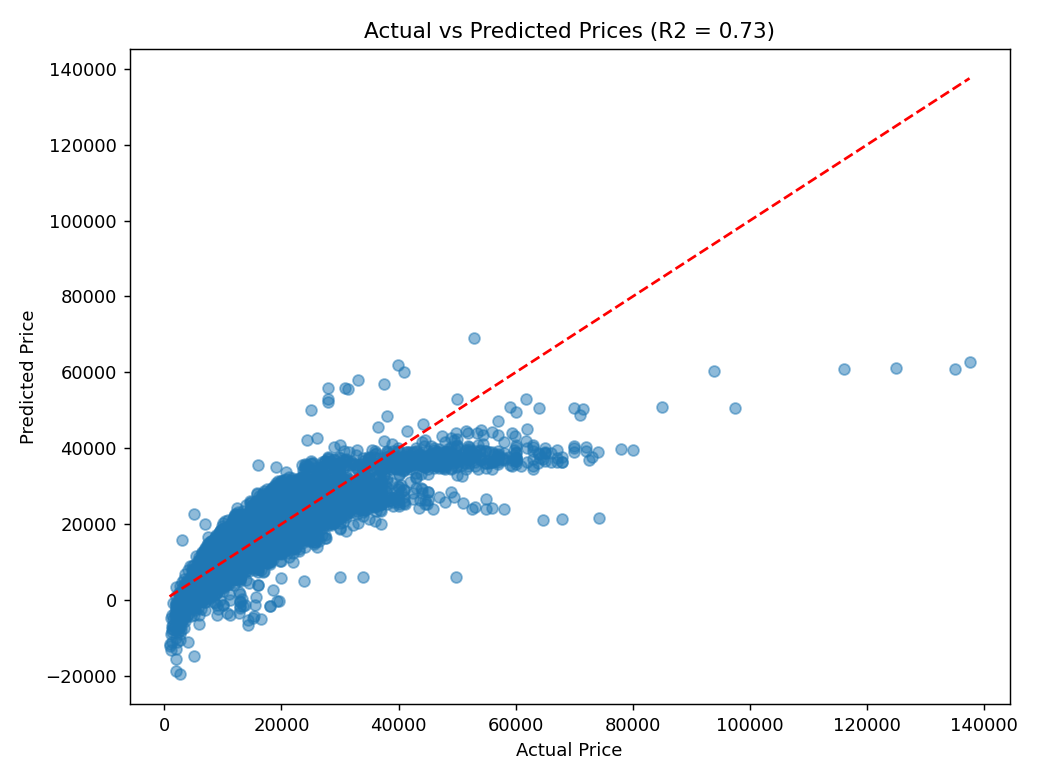
\includegraphics[width=0.55\linewidth]{03_actual_vs_predicted.png}
  \caption{Prix réel vs prédit (jeu de test). Les points suivent globalement la diagonale
    (prédiction parfaite). Le modèle se disperse davantage sur les voitures les plus
    chères (la variance du prix augmente avec sa valeur) : une limite connue de la
    régression linéaire sur des prix bruts.}
  \label{fig:pred}
\end{figure}

\begin{figure}[h]
  \centering
  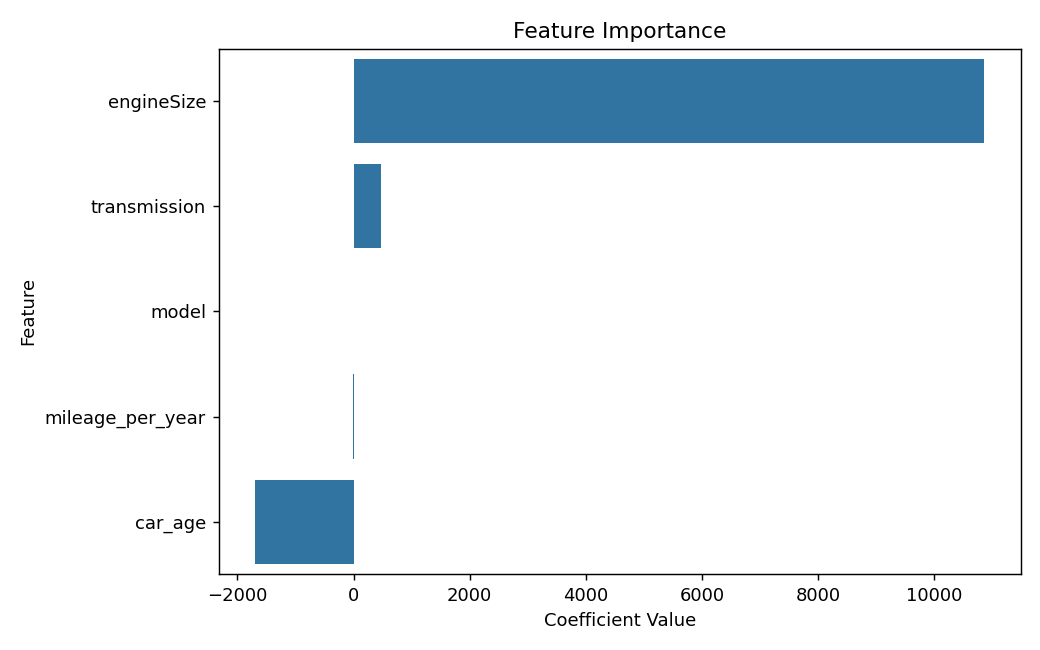
\includegraphics[width=0.6\linewidth]{04_coefficients.png}
  \caption{Coefficients de la régression. La \textbf{cylindrée} fait monter le prix,
    l'\textbf{âge} le fait baisser.}
  \label{fig:coef}
\end{figure}

\medskip
\noindent\textbf{Bug corrigé.} La première version du code \textbf{importait}
\texttt{r2\_score} et \texttt{mean\_squared\_error} \textbf{sans jamais s'en servir} : la
régression ne mesurait donc ni sa qualité ni son erreur. Nous avons ajouté cette
\textbf{évaluation} ($R^2$ + RMSE), qui est le cœur d'un projet de régression. Nous avons
aussi remplacé un \textbf{chemin de fichier codé en dur} par un chemin relatif (le code
tournait seulement sur le PC d'origine).

% =============================================================================
\section{Conclusion}
% =============================================================================

\noindent\textbf{Bénéfices.} Un modèle \textbf{simple et interprétable} explique déjà
\textbf{$\sim$74~\%} de la variance du prix d'une voiture d'occasion. Les leviers sont
clairs : une \textbf{grosse cylindrée} et une \textbf{boîte automatique} font monter le
prix ; l'\textbf{âge} et le \textbf{kilométrage} le font baisser. Nos deux features
maison (\texttt{car\_age}, \texttt{mileage\_per\_year}) portent l'essentiel du signal
temporel.

\medskip
\noindent\textbf{L'enseignement le plus précieux} est venu d'un \textbf{échec} : notre
premier dataset, sur la santé mentale, n'avait aucune corrélation ($\approx 0$) car il
était \textbf{fabriqué}. Des données réelles racontent une histoire ; des données
synthétiques, non.

\medskip
\noindent\textbf{Limites :} (i) \texttt{model} et \texttt{transmission} sont encodées en
nombres, ce qui impose un \textbf{faux ordre} ; (ii) le prix brut rend l'erreur plus
grande sur les voitures chères (Figure~\ref{fig:pred}) ; (iii) marque et carburant ne
sont pas (encore) dans le modèle.

\medskip
\noindent\textbf{Améliorations :} (i) \textbf{one-hot encoding} des catégories ; (ii)
modéliser \textbf{$\log(\text{prix})$} pour stabiliser la variance ; (iii) ajouter
\texttt{Make}, \texttt{fuelType}, \texttt{tax}, \texttt{mpg} ; (iv) tester une régression
régularisée (Ridge/Lasso).

% =============================================================================
\section{List of references}
% =============================================================================

\begin{enumerate}[leftmargin=1.6em]
  \item \textbf{Dataset.} \textit{100,000 UK Used Car Data set} (7 marques fusionnées),
    Kaggle. EDA : https://www.kaggle.com/code/harishkumardatalab/eda-of-multibrand-used-car-dataset?select=used_cars.csv }
    --- CSV utilisé (miroir) : \url{https://github.com/Ajinkya017/Car_Dataset}
  \item \textbf{Cours.} L.\ Fillatre, \textit{Introduction to Data Processing},
    Université Côte d'Azur, Polytech Nice Sophia, 2025-2026 (Lectures 1 à 4).
  \item \textbf{scikit-learn.} Pedregosa et al., \textit{Scikit-learn: Machine Learning
    in Python}, JMLR 12, 2011. \url{https://scikit-learn.org/stable/modules/linear_model.html}
  \item \textbf{pandas.} McKinney, \textit{Data Structures for Statistical Computing in
    Python}, 2010.
  \item \textbf{seaborn.} Waskom, \textit{seaborn: statistical data visualization}, JOSS,
    2021. \url{https://seaborn.pydata.org}
\end{enumerate}

\end{document}
